\documentclass{siamart1116}
\usepackage{amsmath, amssymb}
%\usepackage{amsmath,amssymb,amsfonts,graphicx,amsthm,dsfont}
%\usepackage{listings}
%\usepackage{courier}
\usepackage{enumerate}
%\usepackage{color}
%\usepackage[usenames,dvipsnames]{xcolor}
%\usepackage{hyperref,tikz,mdframed}
%\hypersetup{colorlinks=true,urlcolor=MidnightBlue,citecolor=PineGreen,linkcolor=BrickRed}

% \lstset{
% 	basicstyle=\small\ttfamily,
% 	keywordstyle=\color{blue},
% 	language=python,
% 	xleftmargin=16pt,
% }
\usepackage{algorithmicx}
\usepackage{algpseudocode}% http://ctan.org/pkg/algorithmicx
\usepackage{float}

\textwidth=5.8in
\textheight=9in
\topmargin=-0.5in
\headheight=0in
\headsep=.5in
\hoffset  -.4in
\pagestyle{empty}

\newcommand{\Fp}{\mathbb{F}_p}
\newcommand{\Q}{\mathbb{Q}}
\newcommand{\Z}{\mathbb{Z}}
\newcommand{\kron}[2]{\left(\frac{#1}{#2}\right)}
\newcommand{\Aut}{\mathrm{Aut}}
\newcommand{\End}{\mathrm{End}}
\newcommand{\SO}{\mathrm{SO}}
\newcommand{\SU}{\mathrm{SU}}
\newcommand{\tr}{\operatorname{tr}}
\newcommand{\dee}{\mathrm{d}}
\newcommand{\deee}{\textbf{\text{\emph{d}}}}

\newcommand{\md}[1]{\textcolor{cyan}{#1}}

\newcommand{\TheAuthors}{V. Chen, M. M. Dunlop, A. M. Stuart}

%\newtheorem{theorem}{Theorem}
%\newtheorem{definition}{Definition}

\graphicspath{ {graphics/} }

\title{SURF 2017 Interim Report 1}
\author{\TheAuthors}
\date{}
\begin{document}
\maketitle
\setlength{\unitlength}{1in}
\setlength{\parindent}{0in}

\section{Introduction}
%%%%% will eventually need more background -- definition of graph laplacian, weights, use in unsupervised learning, fiedler vector, etc
In the context of semi-supervised learning, the \textit{clustering} problem refers to attempting to group a set of data or objects into clusters of similar objects. Applications of clustering include image segmentation, social network analysis, and voter classification. We approach the clustering problem from a graph-theoretical point of view, which assigns a node to each data value and edges between nodes to indicate how related the data points are.

Let $Z$ be a set of nodes $\{1, \ldots N\}$. The feature vectors are given by $x : Z \rightarrow \mathbb{R}^d$. $Z' \subset Z$ is a subset of labeled nodes, for which we have label data given by $y : Z' \to \{-1, 1\}$ for binary data, and $y : Z' \to \{1,2,\ldots k\}$ for {\bf $k$-ary} (multiclass) data.


The label model is given by $u$ where $y_l = S(u_l)$ for $l \in Z'$ (with possible corruption by noise). In the case of {\bf binary} data, $y_\ell \in \{\pm 1\}$, and for $v \in \mathbb{R}$,
\[
S(v) = \begin{cases}
1 & v>0\\
0 & v=0\\
-1 & v<0
\end{cases}
\]

In the case of multiclass data, $y_\ell \in \{1, \ldots k\}$, $v \in \mathbb{R}^k$ and
\[
S(v) = \underset{r =1,\ldots,k}{\mathrm{argmax}}\;v_r
\]

Given this problem, one goal is to come up with a classification that best fits the data. Our research group is currently looking at the effectiveness of incorporating Bayesian inference into semi-supervised learning. To view this problem from a Bayesian approach is to attempt to infer the unknown parameters that govern the probability distribution of this unknown. We can be hierarchical with these Bayesian models by having hyperparameters, parameters that govern the distributions of other parameters.

Our focus is on \textit{spectral clustering}, using the clustering properties of the eigenvalues and eigenvectors of the graph Laplacian, a matrix defined on the similarity graph as follows:

Let the similarity graph be $G$ with weights $w_{ij} \ge 0$. A larger weight indicate a higher degree of similarity between the two nodes. Define $\delta_i = \sum_{k=1}^n w_{ij}$. Then, define matrices $W, D$ as:

\[W = w_{ij}, D = \begin{cases} 
\delta_i    & i = j \\
0           & i \neq j 
\end{cases}\]

Then, let $\mathcal{L} = D - W$ denote the unnormalized graph Laplacian on $\mathbb{R}^N$. Denote the eigenbasis of $\mathcal{L}$ by
\begin{equation}
\label{eqn:laplacian}
\mathcal{L}q_j = \lambda_j q_j,\quad j=0,\ldots,N-1.
\end{equation}

The graph Laplacian is important because the eigenvectors corresponding to the smaller eigenvalues are known to hold information about cluster data. In particular, if the graph has ``true'' clusters so that the edges between clusters all have weight 0, then the graph Laplacian would have as many eigenvalues 0 as there are clusters, and the corresponding eigenvectors would be indicators for the clusters \cite{Spectral}. Even if the data is not ideal, the small eigenvectors should hold clustering information. This includes the important Fiedler vector, the second-smallest eigenvector which is useful for bi-partitioning the graph. We assume that the prior distribution of the objective function follows from eigenvectors of the graph Laplacian.

For the Bayesian approach, the prior, likelihood and posterior are defined as follows:
\begin{itemize}
\item[$\mathbb{P}(u)$:] Prior distributed as $N(0,C)$ where the covariance matrix $C = (\mathcal{L} + \tau^2I)^{-\alpha}$. A sample $u$ from the prior can be taken by the following:
\begin{equation}
\label{eqn:prior}
u = \sum_{j=0}^M (\lambda_j + \tau^2)^{-\alpha/2}\xi_j q_j,\quad \xi_j\sim N(0,1) \quad \text{i.i.d.}
\end{equation}

\item[$\mathbb{P}(y|u)$:] Likelihood. For $\gamma > 0$, the likelihood is defined as
\begin{equation}
\label{eqn:likelihood}
\exp(-\Phi(u)) = \displaystyle\exp\left(-\frac{1}{2\gamma^2}\sum_{\ell\in Z'}|y(\ell)-S(u(\ell))|^2\right)
\end{equation}
We choose this likelihood because we assume a normal distribution with mean given by the labeled values $y(l)$ and variance $\gamma^2$.
We will also make use of the $\gamma\to 0$ limit of the likelihood, which is defined as
\begin{equation}
\label{eqn:gammatozero}
\exp(-\Phi(u)) = \begin{cases}
0 & S(u(l)) = y(l) \quad \forall l \in Z'\\
\infty & \text{otherwise}
\end{cases}
\end{equation}

\item[$\mathbb{P}(u|y)$:] Posterior, which by Bayes' theorem is proportional to $\mathbb{P}(u) \mathbb{P}(y | u)$
\end{itemize}

Applications to be considered include the following:
\begin{itemize}
\item The voting records: A data set of the voting records on $16$ votes of $435$ individuals from the U.S. House of Representatives. The data is ordered so that all the representatives from the party are contiguous in the indexing.
\item Two moons: This is a synthetic data set constructed with two half circles in $\mathbb{R}^2$ with radius one. These are embedded in $\mathbb{R}^{100}$, and data points are sampled from the circles with Gaussian noise added to each of the 100 dimensions.
\item MNIST data sets: This data set contains 70,000 images of $28 \times 28$ pixels with handwritten digits $0$ through $9$.
\end{itemize}

My project looks at the effectiveness of different Bayesian hierarchical clustering algorithms. I am implementing these algorithms in Matlab and testing them on the data sets mentioned. The complexity of the models considered will evolve as follows:

\begin{enumerate}[A)]
\item Run fixed $\tau,\alpha, M=N-1$.
\item Learn $\tau,\alpha$; fix $M=N-1$.
\item Learn $\tau,\alpha,M$.
\item $u = \sum_{j=0}^M u_j\xi_j q_j$. Learn $\{u_j\}_{j=0}^M$ with $M$ fixed.
\item Learn $\{u_j\}_{j=0}^M$ and $M$.
\item Multiclass, hierarchical on number of classes.
\end{enumerate}
To learn $\tau, \alpha$, we will assume uniform priors on intervals $U(0, c)$ for constants $c$. For $M$, we will assume an exponentially or algebraically decaying prior with the reasoning that larger $M$ being less likely. We will refer to the hyperparameters as $\theta$.

\section{Approach}
One main goal of this project is to study the effectiveness of different hierarchical models. To do this, I have been understanding the algorithms and implementing them in Matlab. In Matlab, it is easy to visualize the algorithm by plotting the traces of the hyperparameters and the running averages. I can test the algorithms on the data sets and change parameters to see how they affect the clustering effectiveness. I have been using the voting records and the two moons data sets so far. I also made movies of the algorithms running on these data sets by printing figures and using a video-making tool. These movies sometimes start discussions about the effectiveness of the algorithms. Metrics that are useful for comparing the algorithms include the percent classification accuracy, the variance, and the convergence time.

The important next step of this project is to write a test suite for the different algorithms that I have implemented so far. We want to create a figure similar to Figure 13 from \cite{BeLuStZy17}, plotting the classification accuracies of the different algorithms over increasing noise variance in the two moons data set. We would like to see if the hierarchical methods lead to improving classification accuracies.

\section{Algorithms}
When we attempt to sample the posterior distribution in the hierarchical methods, we could use the Gibbs sampler. The basic form of Gibbs sampling has two repeated steps:
\begin{itemize}
\item Update $u^{(n+1)} \sim u|\theta^{(n)}, y$
\item Update $\theta^{(n+1)} \sim \theta|u^{(n+1)}, y$
\end{itemize}
However, we cannot sample the conditional distributions directly, so we could use Markov Chain Monte Carlo (MCMC) indirect sampling methods. With Metropolis-within-Gibbs, we update $u^{(n+1)}$ and $\theta^{(n+1)}$ with MCMC to target these conditional distributions. This is the algorithm that we will be using for the hierarchical algorithms.

\begin{algorithm}
\caption{General pCN adapted from \cite{CoRoStWh13}}
\label{alg:generalpCN}
\begin{algorithmic}
\State{Select $u^{(0)}$. Select $\tau, \alpha$. Select $\beta \in [0, 1]$}
\For{$i = 0$ to $n$}
\State{Sample $\xi$ from the prior distribution given in \cref{eqn:prior}}
\State{Set $v^{(i)} = (1- \beta^2)^{1/2}u^{(i)} + \beta \xi$}
\State{Set $\alpha(u^{(i)} \to v^{(i)}) = \min (1, \exp(\Phi(u^{(i)}) - \Phi(v^{(i)})) )$}
\State{Set $u^{(i+1)} = v^{(i)}$ with probability $\alpha(u^{(i)} \to v^{(i)})$, and set $u^{(i+1)} = u^{(i)}$ otherwise}
\EndFor
\State \Return $u^{(i)}$
\end{algorithmic}
\end{algorithm}

\begin{algorithm}
\caption{Hierarchical on $\tau, \alpha$}
\label{alg:hierarchical_tau_alpha}
\begin{algorithmic}
\State Initialize $\mu^{(0)} = (0, 1, 0, 0, \ldots)$, which is the Fiedler vector written in the orthonormal basis of the eigenvectors
\State Initialize $u^{(0)}$ as $\mu^{(0)}$ expressed in the standard basis.
\State Initialize $\tau^{(0)}, \alpha^{(0)}$. Select $\beta \in [0, 1]$
\State Initialize $\epsilon$
\For{$i = 0$ to $n$}
\State Sample $\xi$ from the prior distribution and expressed in the eigenbasis \Comment{$u|y, \tau, \alpha$}
\State Set a proposal $\nu^{(i)} = (1- \beta^2)^{1/2}\mu^{(i)} + \beta \xi$
\State Compute $v^{(i)}$ as $\nu^{(i)}$ in the standard basis
\State Set $u^{(i+1)} = v^{(i)}$ and $\mu^{(i+1)} = \nu^{(i)}$ with probability $\min (1, \exp(\Phi(u^{(i)}) - \Phi(v^{(i)})) )$

\State Set a proposal $t^{(i)} = \tau^{(i)} + \epsilon \zeta^{(i)}$ for $\zeta^{(i)} \sim N(0, 1)$ \Comment{$\tau|y,u,\alpha$}
\State Set $\tau^{(i+1)} = t^{(i)}$ with probability given by the ratio between the joint posterior functions on $u, \tau, \alpha$: $f(\mu^{(i+1)}, t^{(i)}, \alpha^{(i)})/f(\mu^{(i+1)}, \tau^{(i)}, \alpha^{(i)})$ (using the eigenbasis representation to simplify computation)

\State Set a proposal $a^{(i)} = \alpha^{(i)} + \epsilon \zeta^{(i)}$ for $\zeta^{(i)} \sim N(0, 1)$ \Comment{$\alpha|y,u,\tau$}
\State Set $\alpha^{(i+1)} = a^{(i)}$ with probability given by $f(\mu^{(i+1)}, \tau^{(i+1)}, a^{(i)})/f(\mu^{(i+1)}, \tau^{(i+1)}, \alpha^{(i)})$
\EndFor\\
\Return $u^{(i)}, \tau^{(i)}, \alpha^{(i)}$
\end{algorithmic}
\end{algorithm}

\begin{algorithm}
\caption{Non-centered parameterization: sampling $\xi, \tau, \alpha$}
\label{alg:xi_tau_alpha}
\begin{algorithmic}
\State Choose $\xi^{(0)} \in \mathbb{R}^N, \alpha^{(0)}, \tau^{(0)} > 0, \beta \in (0, 1]$ and $\epsilon_1, \epsilon_2 > 0$.
\State Define \[ g(\xi,\tau,\alpha) \propto \exp\left( -\Phi(T(\xi,\tau,\alpha))-\frac{1}{2}\langle \xi,\xi \rangle + \log(\pi_0(\tau,\alpha)) \right)\]
\For{$k=0$ to $S$}
\State Propose $\hat\xi^{(k)} = (1-\beta^2)\xi^{(k)} + \beta \zeta^{(k)}$, $\zeta^{(k)} \sim N(0, I)$
\State Make transition $\xi^{(k+1)} \to \hat\xi^{(k)}$ with probability
\[ A(\xi^{(k)} \to \hat\xi^{(k)}) = \min\{1, \exp\left(\Phi(\xi^{(k)},\tau^{(k)},\alpha^{(k)}) - \Phi(\hat\xi^{(k)},\tau^{(k)},\alpha^{(k)})\right) \}\]

\State Propose $\hat\tau^{(k)} = \tau^{(k)} + \epsilon_1 \rho^{(k)}, \rho^{(k)} \sim N(0,I)$
\State Make transition $\tau^{(k+1)} \to \hat\tau^{(k)}$ with probability
\[ A(\tau^{(k)} \to \hat\tau^{(k)}) = \min\{1, \frac{g(\xi^{(k+1)},\hat\tau^{(k)},\alpha^{(k)})}{g(\xi^{(k+1)},\tau^{(k)},\alpha^{(k)})} \}\]

\State Propose $\hat\alpha^{(k)} = \alpha^{(k)} + \epsilon_2 \sigma^{(k)}, \sigma^{(k)} \sim N(0,I)$
\State Make transition $\alpha^{(k+1)} \to \hat\alpha^{(k)}$ with probability
\[ A(\alpha^{(k)} \to \hat\alpha^{(k)}) = \min\{1, \frac{g(\xi^{(k+1)},\tau^{(k+1)},\hat \alpha^{(k)})}{g(\xi^{(k+1)},\tau^{(k+1)},\alpha^{(k)})} \}\]
\EndFor
\State \Return $\{ T(\xi^{(k)},\tau^{(k)},\alpha^{(k)}), \tau^{(k)}, \alpha^{k} \}$
\end{algorithmic}
\end{algorithm}




\section{Work accomplished}
So far, I have implemented models A and B in Matlab. I implemented a pCN algorithm first introduced in \cite{BeRoStVo08}, given in \cref{alg:generalpCN}.
I applied this model on the voting records data set and could get clustering at about 85\% accuracy. One final clustering obtained is shown in \cref{fig:mcmc_gamma_final}.
\begin{figure}[!htb]
\label{fig:mcmc_gamma_final}
\caption{Average of signs of $u$ indicate the final clustering}
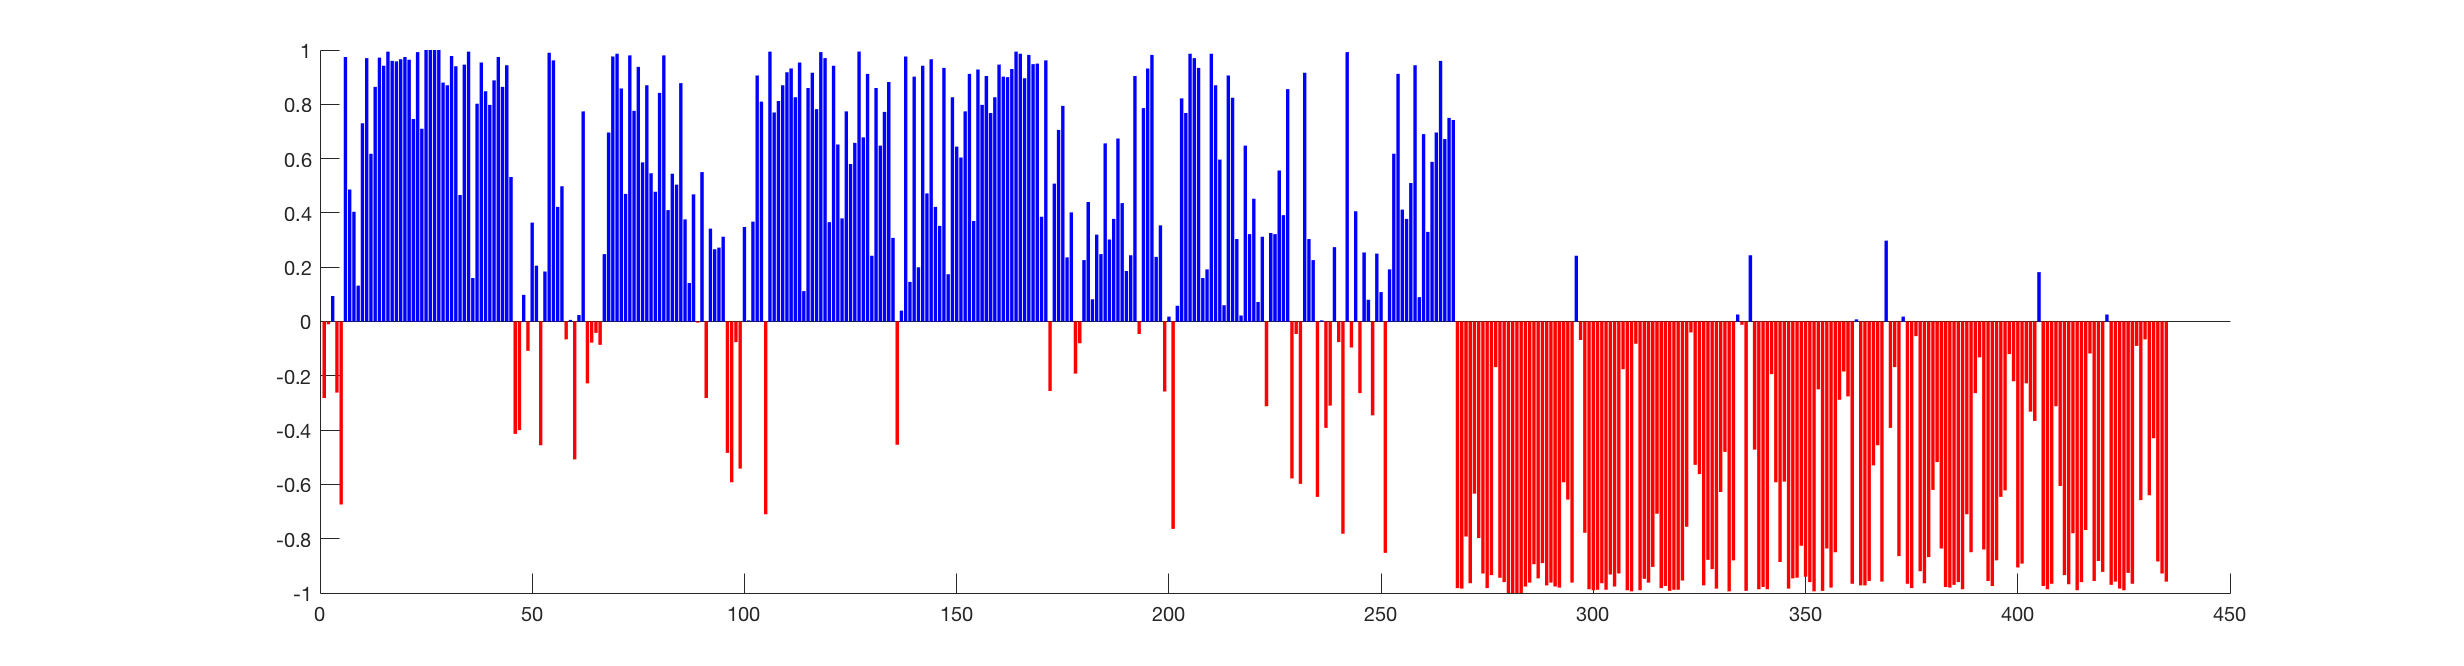
\includegraphics[width = \linewidth]{mcmc_gamma/manycorrect_clustering.png}
\end{figure}

Next, I implemented an algorithm for model B, given in \cref{alg:hierarchical_tau_alpha}. We are now being hierarchical about the values of $\tau$ and $\alpha$, so we refer to the Metropolis-within-Gibbs method described above.

I ran experiments with this algorithm on the voting records data but plotting the traces of $\tau, \alpha$ and looking at the final average suggested that the Markov chain was not converging. After discussing with my mentor, we decided that the problem was in part due to the irregularity of the larger eigenvectors, perhaps because of the accuracy of Matlab's eig solver. Truncating the list of eigenvectors to only consider the first 50 seemed to help the problem, and we were able to observe better clustering. See \cref{fig:centered_voting_avg}, \cref{fig:centered_voting_tau}.

\begin{figure}[H]
\begin{minipage}{0.48\textwidth}
    \caption{\label{fig:centered_voting_avg} \cref{alg:hierarchical_tau_alpha} final average after truncating eigenvectors}
    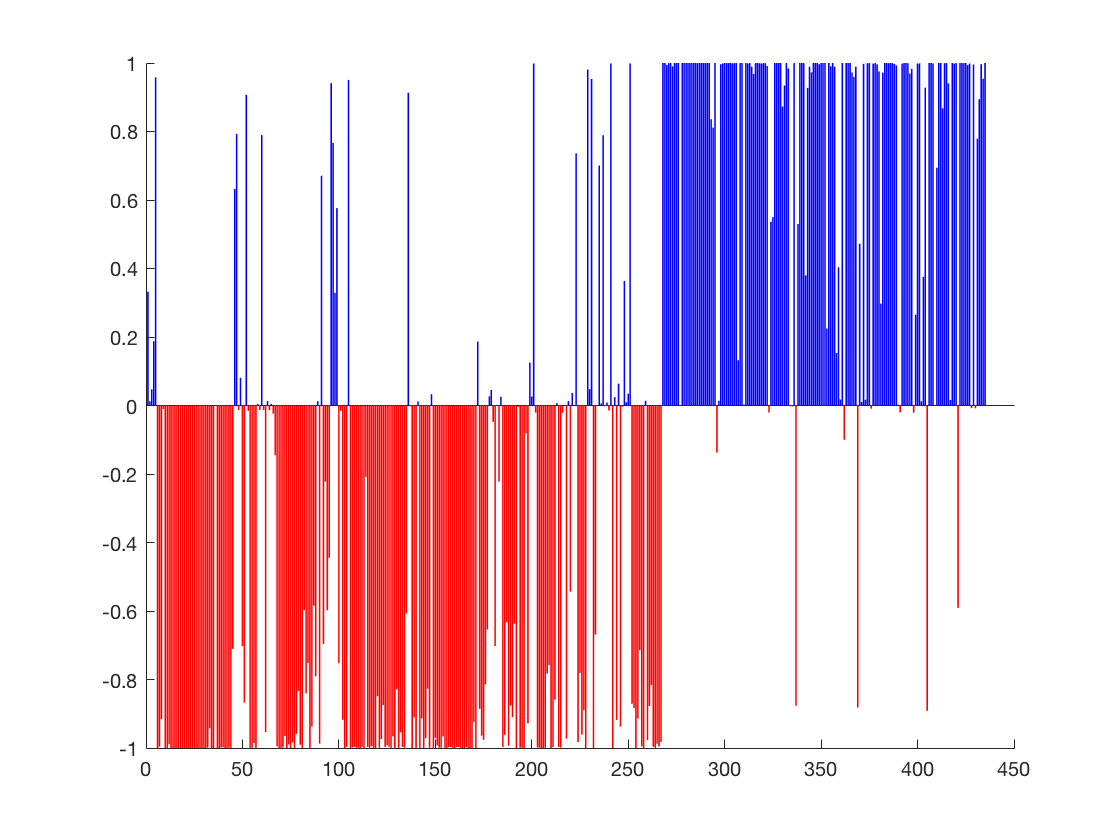
\includegraphics[width=\linewidth]{centered/final_avg.png}
\end{minipage}\hfill
\begin{minipage}{0.48\textwidth}
    \caption{\label{fig:centered_voting_tau} Trace of $\tau$}
    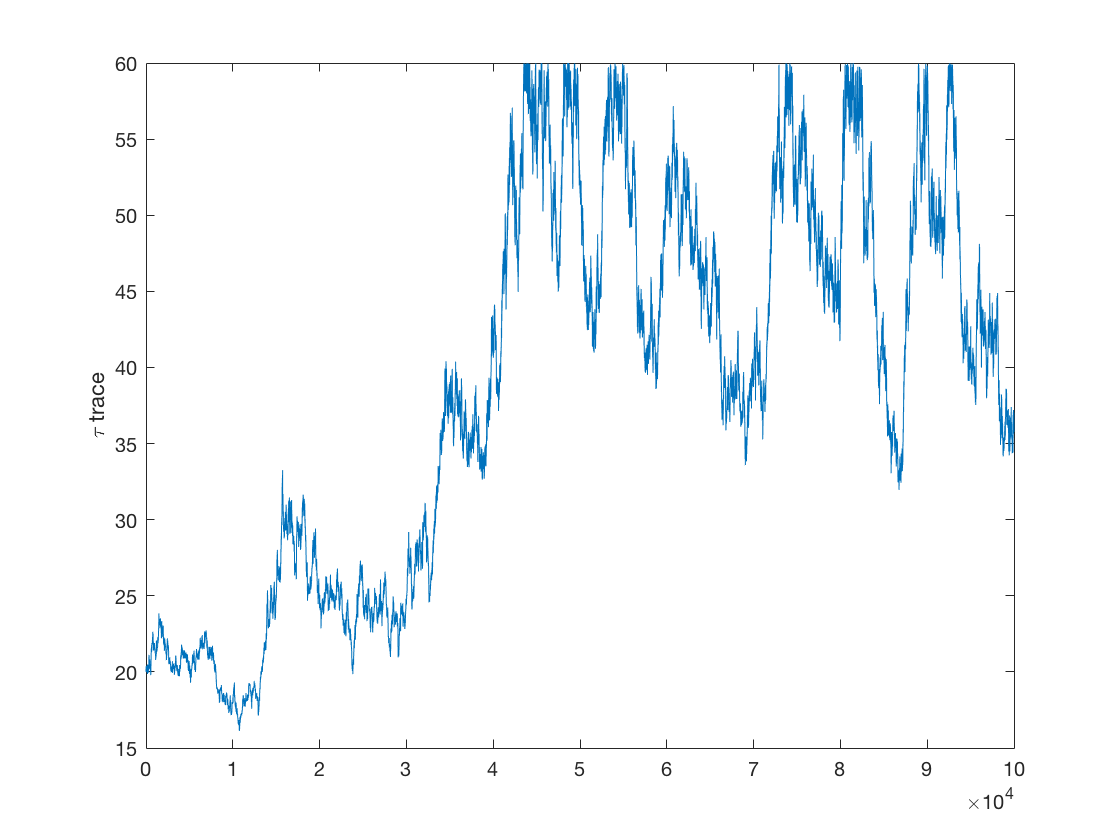
\includegraphics[width=\linewidth]{centered/trace_tau.png}
\end{minipage}
\end{figure}

We also looked at a different parameterization for being hierarchical about $\tau$ and $\alpha$. \cref{alg:xi_tau_alpha} is non-centered compared to the previous algorithm.

This non-centered algorithm seems to converge faster than the centered one, and truncation of the eigenvectors is not necessary. See \cref{fig:noncentered_voting_avg}, \cref{fig:noncentered_voting_tau}

\begin{figure}[H]
\begin{minipage}{0.48\textwidth}
    \caption{\label{fig:noncentered_voting_avg}\cref{alg:xi_tau_alpha} final average}
    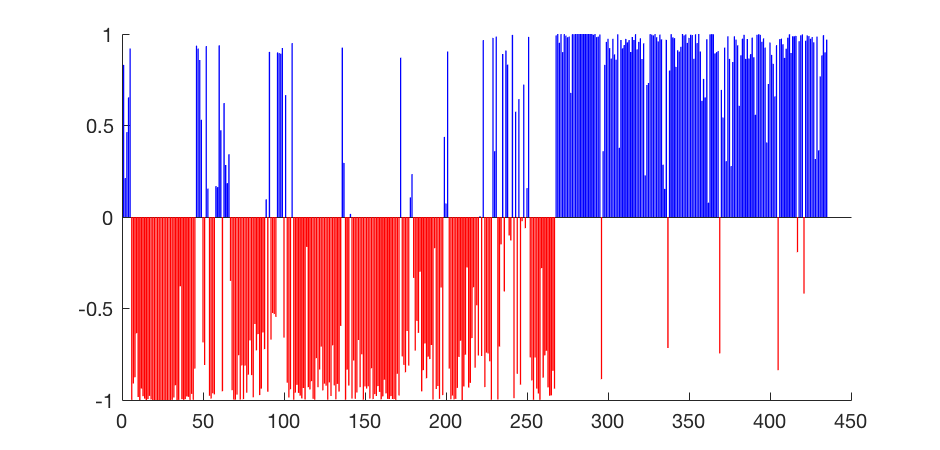
\includegraphics[width=\linewidth]{noncentered/final_avg.png}
\end{minipage}\hfill
\begin{minipage}{0.48\textwidth}
    \caption{\label{fig:noncentered_voting_tau} Trace of $\tau$}
    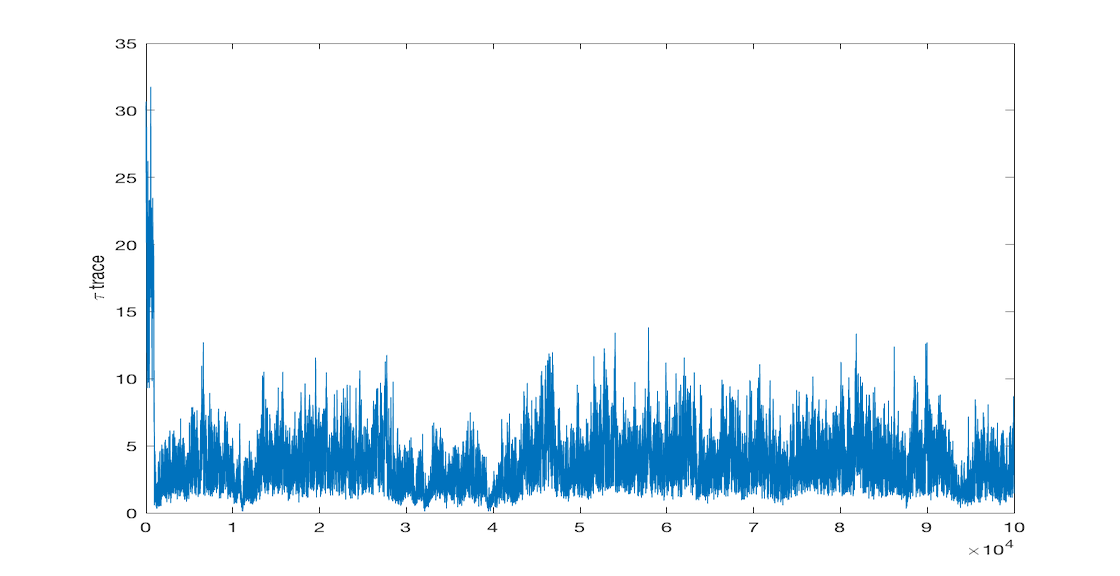
\includegraphics[width=\linewidth]{noncentered/trace_tau.png}
\end{minipage}
\end{figure}

Using these algorithms, I also ran experiments to cluster the two-moons data set. We explored using the self-tuning Laplacian, which was introduced in \cite{SelfTuning}. This Laplacian matrix has weights that infer the local spatial scale from the data, removing the need to choose a fixed length-scale parameter. The use of this self-tuning Laplacian in the two-moons data set seems to encode more information in the eigenvectors. Compare \cref{fig:moon_laplacian_un} with \cref{fig:moon_laplacian_selftuning}. 

\begin{figure}[!htb]
    \begin{minipage}{0.48\textwidth}
        \centering
        \caption{\label{fig:moon_laplacian_un} First eigenvectors of unnormalized Laplacian for intertwined moons data}
        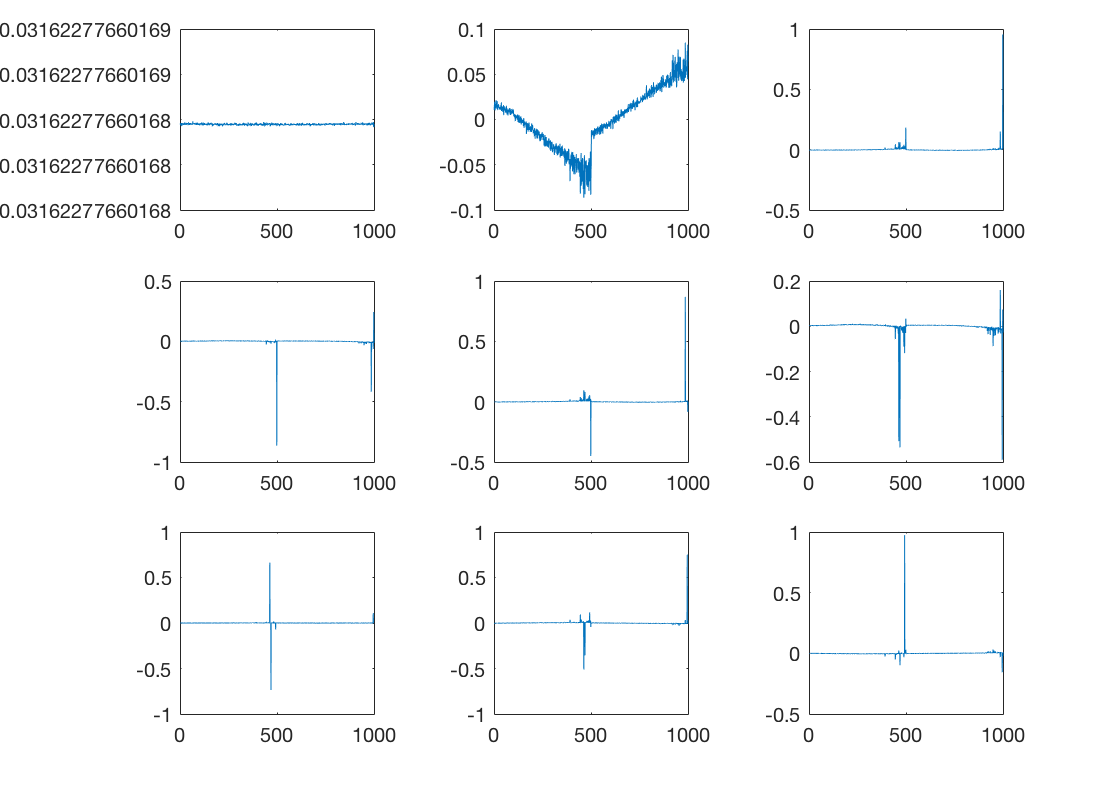
\includegraphics[width=\linewidth]{graphics/moon_laplacian_un.png}
    \end{minipage} \hfill
    \begin{minipage}{0.48\textwidth}
        \centering
        \caption{\label{fig:moon_laplacian_selftuning} First eigenvectors of unnormalized self-tuning Laplacian for intertwined moons data}
        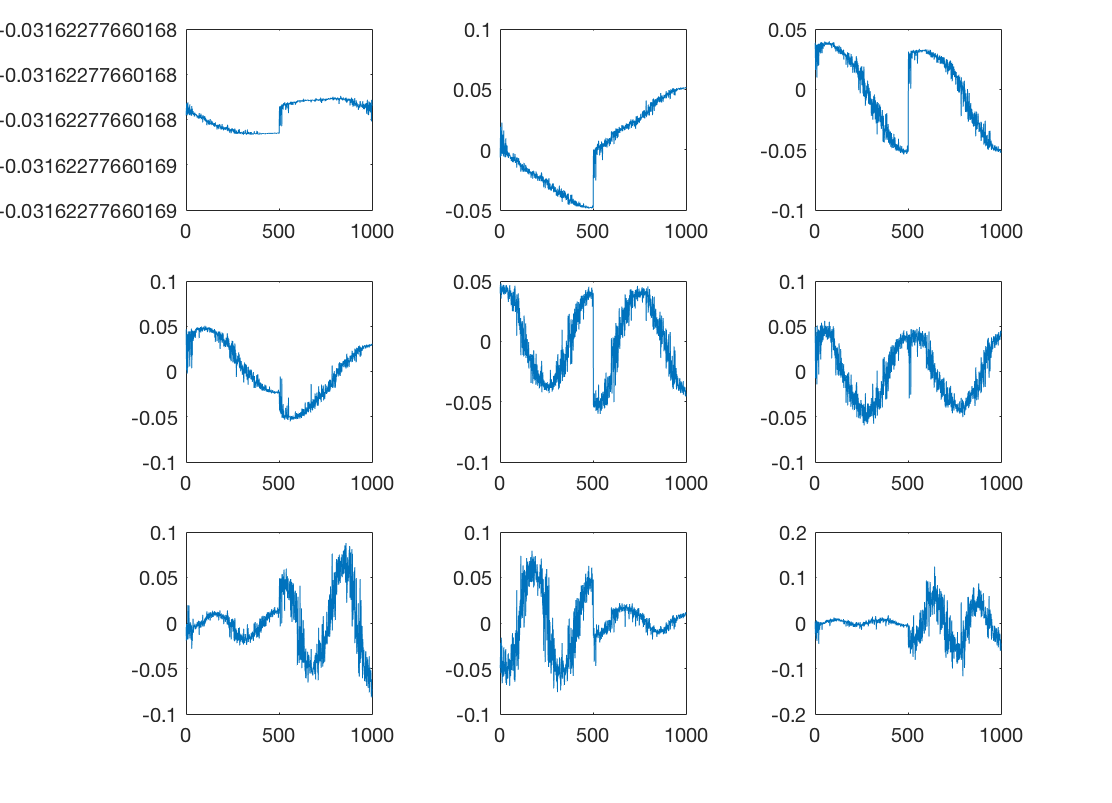
\includegraphics[width=\linewidth]{graphics/moon_laplacian_selftuning.png}
    \end{minipage}
\end{figure}

Compare the results from the centered, truncated algorithm and the non-centered self-tuning algorithm in \cref{fig:moon_centered_avg}, \cref{fig:moon_noncentered_avg}, \cref{fig:moon_centered_trace_tau}, \cref{fig:moon_noncentered_trace_tau}, \cref{fig:moon_centered_trace_alpha}, \cref{fig:moon_noncentered_trace_alpha}.
\begin{figure}[H]
    \begin{minipage}{0.48\textwidth}
        \centering
        \caption{\label{fig:moon_centered_avg} Centered, truncated algorithm, final average}
        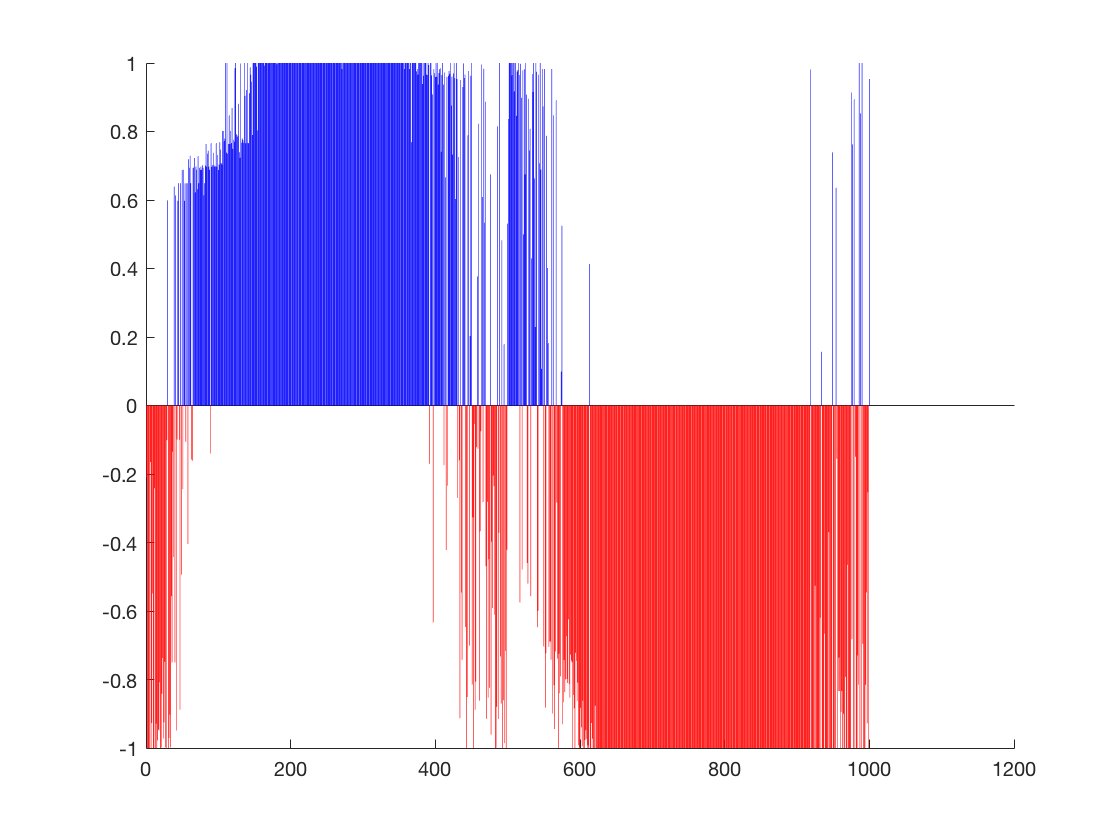
\includegraphics[width=\linewidth]{graphics/moons/centered_truncated/final_avg.png}
    \end{minipage} \hfill
    \begin{minipage}{0.48\textwidth}
        \centering
        \caption{\label{fig:moon_noncentered_avg} Non-centered, self-tuning algorithm, final average}
        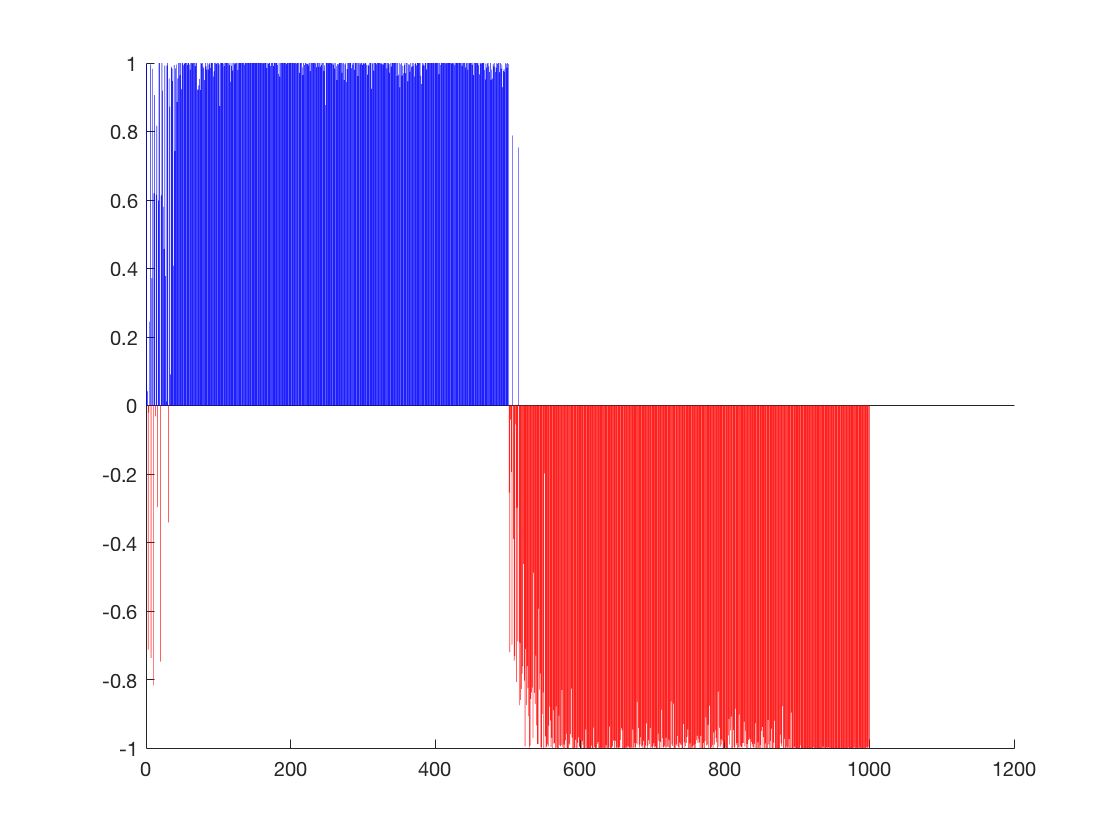
\includegraphics[width=\linewidth]{graphics/moons/noncentered_selftuning/final_avg.png}
    \end{minipage}
\end{figure}

\begin{figure}[H]
    \begin{minipage}{0.48\textwidth}
        \centering
        \caption{\label{fig:moon_centered_trace_tau} Centered, truncated algorithm, trace $\tau$}
        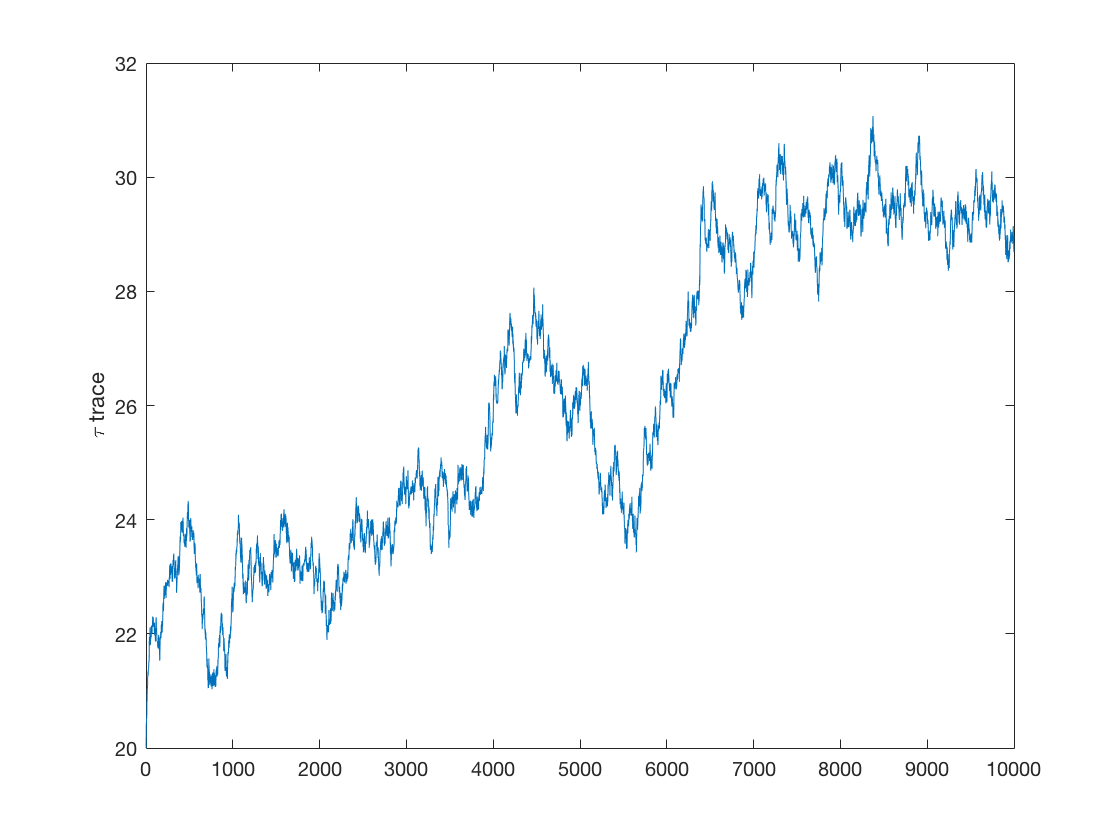
\includegraphics[width=\linewidth]{graphics/moons/centered_truncated/trace_tau.png}
    \end{minipage} \hfill
    \begin{minipage}{0.48\textwidth}
        \centering
        \caption{\label{fig:moon_noncentered_trace_tau} Non-centered, self-tuning algorithm, trace $\tau$}
        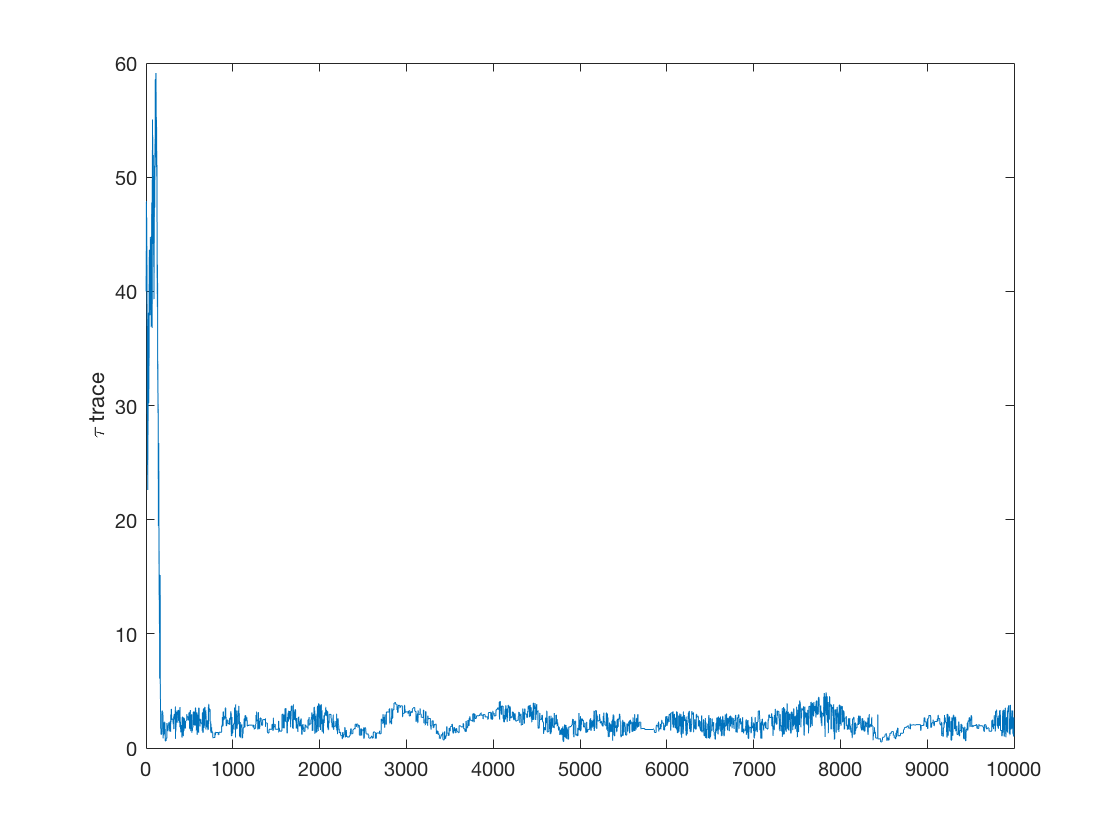
\includegraphics[width=\linewidth]{graphics/moons/noncentered_selftuning/trace_tau.png}
    \end{minipage}
\end{figure}

\begin{figure}[H]
    \begin{minipage}{0.48\textwidth}
        \centering
        \caption{\label{fig:moon_centered_trace_alpha} Centered, truncated algorithm, trace $\alpha$}
        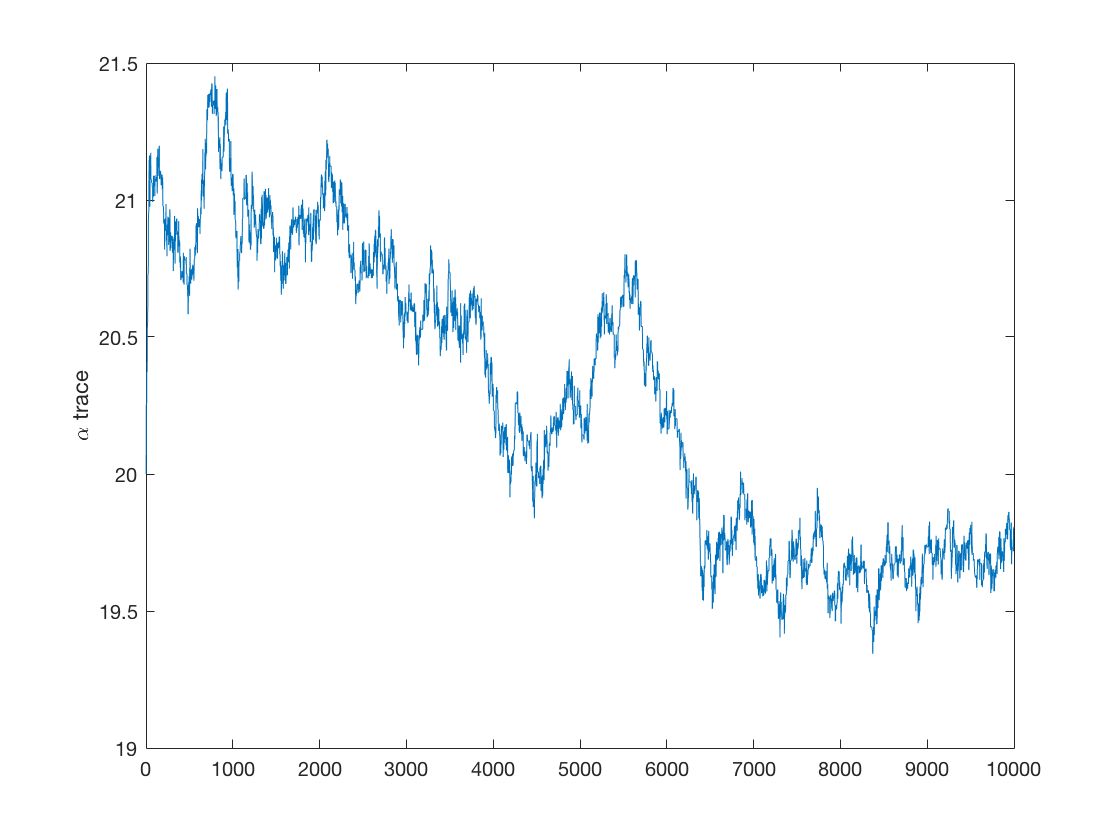
\includegraphics[width=\linewidth]{graphics/moons/centered_truncated/trace_alpha.png}
    \end{minipage} \hfill
    \begin{minipage}{0.48\textwidth}
        \centering
        \caption{\label{fig:moon_noncentered_trace_alpha} Non-centered, self-tuning, trace $\alpha$}
        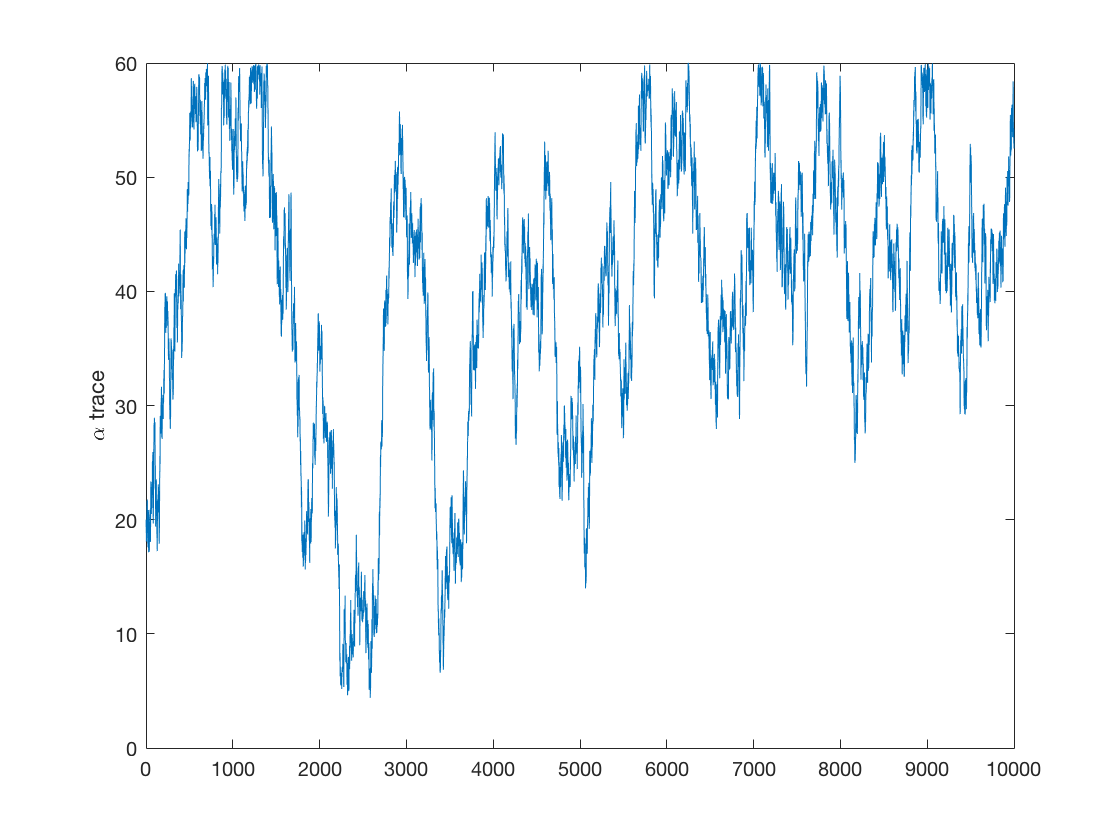
\includegraphics[width=\linewidth]{graphics/moons/noncentered_selftuning/trace_alpha.png}
    \end{minipage}
\end{figure}

Notice the convergence of $\tau$ and its low variance in the samples for the non-centered self-tuning algorithm. The distribution of $\tau$ is different between the two algorithms because truncating the number of eigenvectors affects the distribution of the posterior.

\section{Challenges}
Some common issues that I encountered are bugs in my Matlab code. Some of these bugs included overflow or underflow of ratios, when both numerator and denominator are very large or very small. To improve accuracy, I implemented these ratios as the difference between $\log$s, and took the $\exp$ of the result at the end. I became used to using Matlab's debugger to step through line-by-line and isolate the mistakes.

Another challenge was trying to get \cref{alg:hierarchical_tau_alpha}, the centered hierarchical algorithm, to perform well. The first implementation of that algorithm gave traces of the hyperparameters with low mixing and poor clustering of the voting records. Allowing for large ranges for $\tau$ and $\alpha$ did not solve the problem as the MCMC seemed to find one value of $\tau$ and stay stuck at that value. To try to debug the code, I re-implemented the algorithm using more of the linear algebra functionality of Matlab and improved the readability. This did not solve the problem, and my co-mentor suggested that the problem might have to do with the eig solver of Matlab failing for larger eigenvalues. We tested this by truncating the list of eigenvectors from $435$ down to only $50$, and the results, as mentioned above, were better. Since this fix is specific to these data sets, moving forward I anticipate that there may be more challenges with this algorithm.

We have also found that $\tau$ seems to have much lower variance than $\alpha$, and it is difficult to see if $\alpha$ has converged. I have tried looking at histograms for $\alpha$ and seeing if the distribution is different from the starting distribution, but the convergence of $\alpha$ could continue to be a problem.

\section{Additional resources}
My project is mostly done on my computer, my notebook, and a whiteboard. Most likely, I will not require additional resources other than references to papers and books to read to understand the algorithms.

\bibliographystyle{siamplain}
\bibliography{references}
\end{document}